\begin{frame}
\frametitle{Introduction of CG Term}

\begin{columns}

    % Image on the left
    \begin{column}{0.48\textwidth}
        \centering
        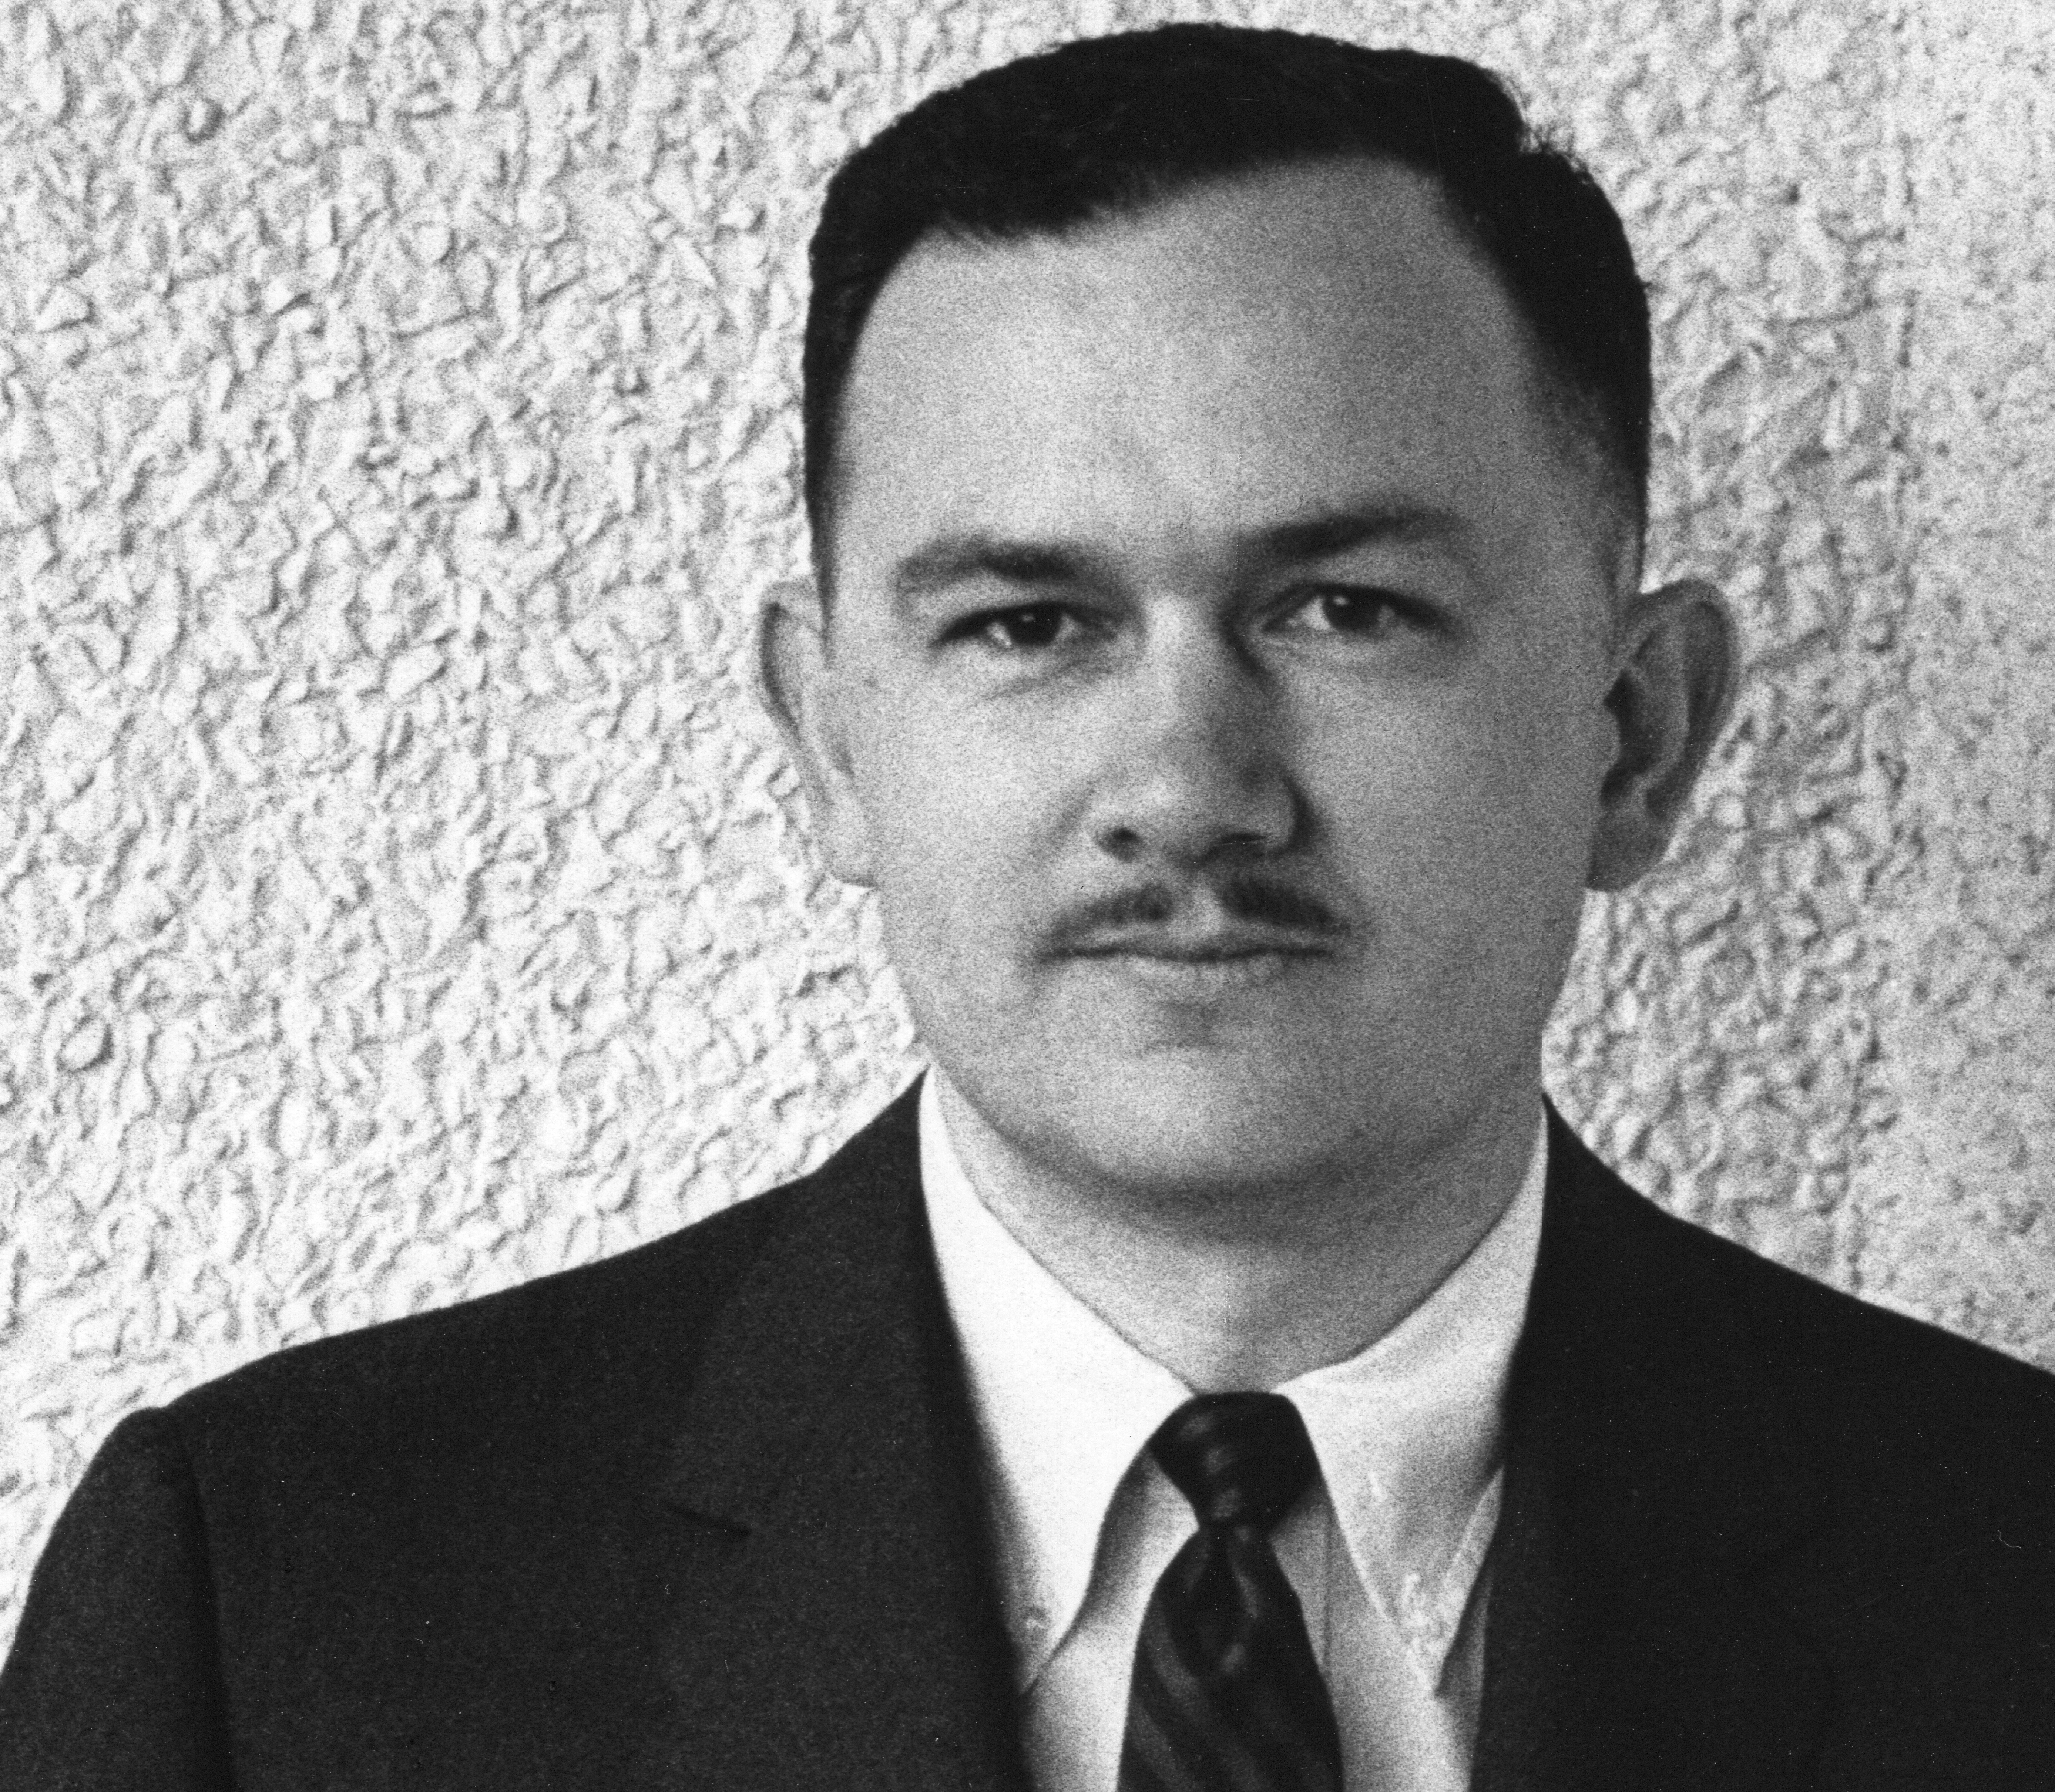
\includegraphics[width=\linewidth]{assets/WilliamFetter.jpg}
    \end{column}

    % Text on the right
    \begin{column}{0.48\textwidth}
        William A. Fetter coined the CG term while he was working as a graphics designer at Boeing in 1960.
    \end{column}

\end{columns}

\end{frame}
%==================================================================================
\begin{frame}
\frametitle{First Boeing Man}

He was the first person to represent the human figure as a 3D model.
He created the model to study ergonomics and pilot visibility in aircraft cockpits.

\vspace{0.5cm}

\begin{columns}

    \begin{column}{0.48\textwidth}
        \centering
        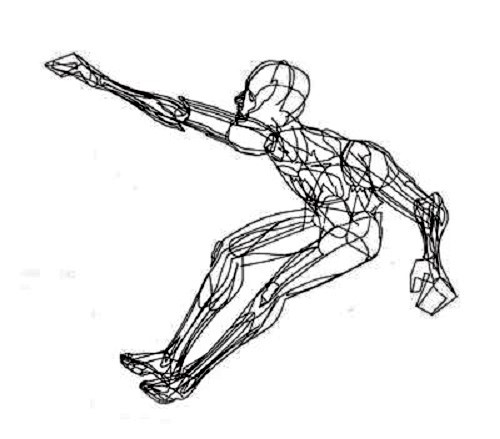
\includegraphics[width=\linewidth]{assets/BoeingMan.jpg}
        
        \small First Boeing Man 
    \end{column}

    \begin{column}{0.48\textwidth}
        \centering
        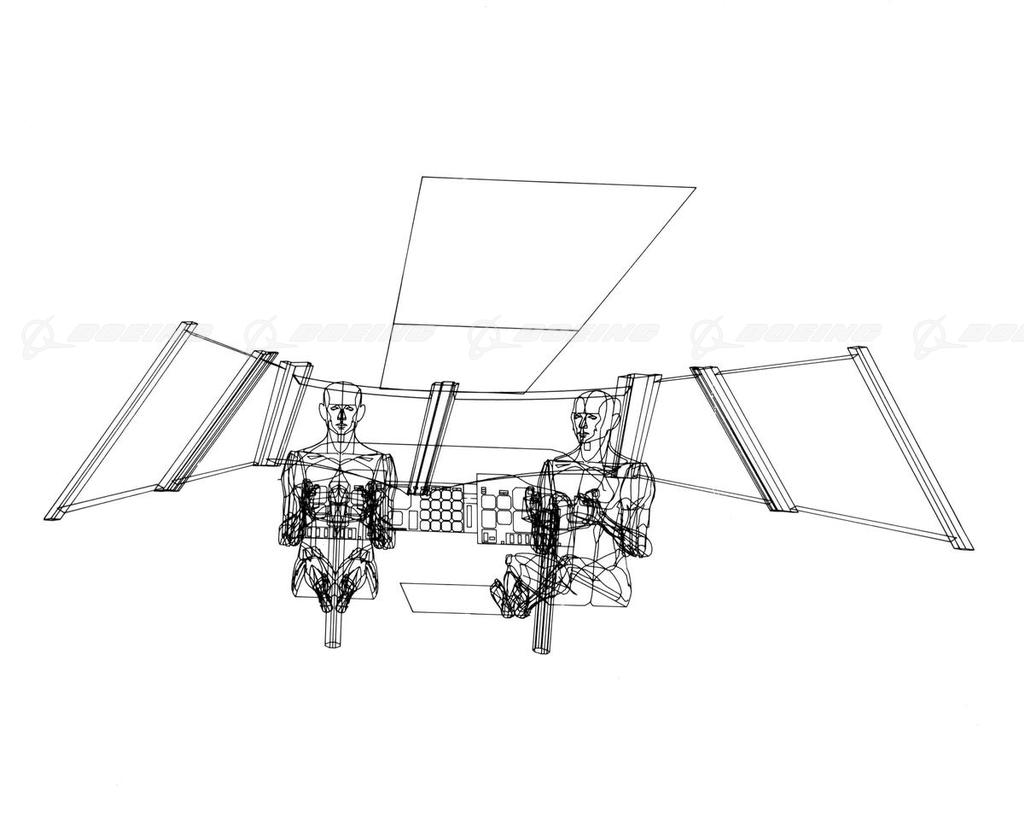
\includegraphics[width=\linewidth]{assets/pilots.jpg}
        
        \small Pilots visibility in cockpit
    \end{column}

\end{columns}

\end{frame}
%==================================================================================